
% Desc: Stage user manual
% Author: Richard Vaughan, Andrew Howard
% Date: 10 Jun 2002
% CVS: $Id: stage.tex,v 1.22 2004-08-23 18:47:28 rtv Exp $

\documentclass[letter,11pt,twoside]{report}

% this one apparently fixes the < and > chars
\usepackage[T1]{fontenc}
\usepackage{subfigure}
\usepackage{times}
\usepackage{tabularx}

% why did we need this?
%\usepackage{verbatim}
% make all captions small and slanted
\usepackage[small,sl]{caption}
\usepackage{fullpage}
%\usepackage{epsf}
\usepackage{epsfig}
\usepackage{graphicx}
% add nifty DRAFT watermark thingy in PS
\usepackage{draftcopy}

% A nice environment for displaying command line args (AH)
\newenvironment{xarg}[1]{\noindent{\tt #1}\\\hspace*{2em}\begin{minipage}[t]{5in}}{\end{minipage}\vspace*{1em}}

\def\VERSION {1.5}
\def\HOMEPAGE {{\tt http://playerstage.sourceforge.net}}
\def\SFPAGE {{\tt http://sourceforge.net/projects/playerstage/}}

\begin{document}

\setcounter{page}{0}
\pagenumbering{roman}

\titlepage

 \begin{tabular}{lcr}
   \begin{tabular}{c}
        Player/Stage project\\
         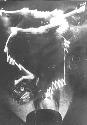
\includegraphics{notext_ps_logo}
    \end{tabular}
   &
   \hspace{5cm}
   &
   \begin{tabular}{r}
     {\bf Autonomy Laboratory}\\
     Simon Fraser University\\
     Burnaby, British Columbia, Canada\\
     \vspace*{2em}\\
     {\bf USC Robotics Laboratory}\\
     University of Southern California\\
     Los Angeles, California, USA\\
     \vspace*{2em}\\
     {\bf Stanford Robotics Laboratory}\\
     Stanford University\\
     Stanford, California, USA\\
   \end{tabular}
 \end{tabular}


  \vspace{4cm}  
  \centerline{ \Huge{Stage}}
  \vspace{0.5cm}
  \centerline{\large{Version \VERSION{} User Manual}}
  \vspace{2cm}
  \centerline{\large Richard T.~Vaughan \\ Andrew Howard \\ Brian P.~Gerkey}
  \vspace{1cm}

  \centerline{This document may not contain the most current documentation on}
  \centerline{Stage.  For the latest documentation, consult the Player/Stage homepage:}
  \centerline{\HOMEPAGE}

  \vspace{4cm}

 \centerline{\today}

\tableofcontents
%\newpage

%\listoffigures
%\newpage
%\listoftables
%\newpage

% reset page number to start with 1
\setcounter{page}{0}
\pagenumbering{arabic}


\chapter{Introduction}

\section{ Stage and the Player/Stage Project}

The Player/Stage Project produces software tools to support research
in autonomous robotics, sensor systems and animats (artificial
creatures). Stage is a robot simulator. It models a population of
mobile robots, sensors and environmental objects in a two-dimensional
world. Stage is designed with multi-agent systems in mind, so it
provides fairly simple, computationally cheap models of lots of
devices rather than attempting to emulate any device with great
fidelity. This design is intended to be useful compromise between the
conventional high-fidelity robot simulations, the minimal simulations
described by Jakobi\cite{jakobi:radical}, and the grid-world
simulations common in animat research\cite{wilson:animat}. We intend
Stage to be just realistic enough to enable users to move controllers
between Stage robots and real robots, while still being fast enough to
simulate large populations. We also intend Stage to be comprehensible
to undergraduate students, yet sophisticated enough for professional
reseachers.

Stage devices are usually controlled through \emph{Player}; a
networked robot server. Player provides a convenient interface to a
set of device drivers for real robots and sensors. Stage simulates a
population of devices and makes them available thorugh Player. Users
write robot controllers and sensor algorithms as `clients' to the
Player `server'. Typically, clients cannot tell the difference between
the real robot devices and their simulated Stage equivalents (unless
they try very hard). We have found that robot controllers developed as
Player clients controlling Stage robots will work with little or no
modification with the real robots and vice versa. With a little care,
the same binary program can often control Stage or real robots without
even being recompiled. Thus the Player/Stage system allows rapid
prototyping of controllers destined for real robots. Stage can also be
very useful by simulating populations of realistic robot devices you
don't happen to own.
  
Various sensors and actuators are provided, including sonar or
infrared rangers, scanning laser rangefinder, color-blob tracking,
fiducial tracking and mobile robot bases with odometry. {\bf Note:
Some models from previous versions may not yet be available in this
release, but we're working on them. Let us know which ones you need.}

\section{How to get Stage and related software}

The main source for all things Player/Stage is the project
homepage:\\\\ \indent
\HOMEPAGE\\

\noindent Access to source code releases, access to the CVS
development tree, bug tracking, user mailing lists, etc.~ is
available from the Sourceforge project management page:\\\\\indent
\SFPAGE\\

\noindent The current release is available as the source tarball
Stage-<version>.src.tgz at:\\\\ \indent
http://sourceforge.net/project/showfiles.php?group\_id=42445\\

Where \verb+<version>+ indicates the most recent (i.e. largest)
version number you find at the site.  Previous versions were
significantly different; this manual does not apply to them.

\section{What's in the Package?}

In the release tarball you will find:
\begin{itemize}
\item Documentation, including this manual and release notes (in the
  directory \verb'docsrc').
\item C source code for 'stage' the simulation engine (in \verb'src').
\item C and C++ code for the 'libStage' client library (in \verb'src').
\item Example worldfiles and bitmaps (in \verb'worlds' ).
\item Example Player configuration files for using Player with
Stage(in \verb'config').
\end{itemize}

\section{Platform and Requirements}

Stage was developed and tested under Linux kernel 2.4 and 2.6,
glibc-2.2 and OS X.3. The C and C++ source code is reasonable
ANSII/POSIX so it often compiles elsewhere. No promises, but people
have found it to work on a variety of set-ups. Some people have had
success with Microsoft Windows and CYGWIN, but this is not currently a
target tested by the maintainers. Using a UNIX-like system will
probably be easier for you. Player/Stage programs are Free Software
too, so using them with Linux can cost you \$0, freeing up your budget
to do more science for the benefit of society and/or your company.

\subsection{Dependencies}

\begin{itemize}
\item libRTK2 [the Player/Stage GUI toolkit \HOMEPAGE] 
\item GTK+ (packaged with GNOME)
\item glib (usually packaged with GTK+)
\item pkg-config (usually packaged with GTK+)
\item X11R6 (usually installed by default on Linux, Solaris and BSD,
  optional free download on OS X)
\end{itemize}

Optional, but very useful, and recommended if you ever want to use
controller code on real robots:
\begin{itemize}
\item Player [\HOMEPAGE]
\end{itemize}

\section{Ownership and Licensing}

Stage is released under the GNU General Public License. Stage
programs, images, examples, source code and documentation are ownded
and copyrighted by their authors. The authors, roughly in order of
date of contribution, are:

\begin{itemize}
\item[] Richard Vaughan [vaughan@sfu.ca]
\item[] Kasper Stoy 
\item[] Andrew Howard [ahoward@robotics.usc.edu]
\item[] Brian Gerkey [gerkey@robotics.stanford.edu]
\item[] Boyoon Jung 
\item[] Jakob Fredslund
\item[] Esben \O{}sterg\aa{}rd
\item[] Jason K~ Douglas
\item[] Kim Jinsuck
\item[] Gabe Sibley
\item[] Dave Naffin
\end{itemize}

The list of authors above is a partial one: the code itself contains
the definitive ownership and licensing statements.

See your name here by contributing devices, superior algorithms,
bugfixes, examples, docs, etc. If you contributed to Stage and we
forgot to add you here, either add yourself here (if you have CVS
write access) or let us know and we'll be happy to correct the
ommision.

\section{Bugs and feedback}

This is constantly evolving research software. It is bound to contain
bugs, despite developer and user testing. Stage is occasionally
overhauled, revealing or introducing new bugs. If you find something
that appears to be a bug, or if some aspect of Stage's behavior seems
wrong or non-intuitive, let us know. If you have a problem, please
first check the website and bug tracking logs - hundreds of questions
have been answered there. If you can't find an answer there,{\emph use
the bug tracker} to tell us about the problem. Better still, fix it
and send us the patch. To stay in touch with the developers and other
users, join the mailing lists.

When submitting bugs, include as much information as possible,
including the Stage version, OS type and version, and any output
messages.  A detailed description of what happened will enable us
(hopefully) to repeat and analyze the problem.  Of course, there is NO
WARRANTY on this software, and no guarantee that we will fix your
problem.  Remember, you didn't pay for this stuff\footnote{If you {\em
did} pay for this stuff: thanks, and please ignore the referring
paragraph. If you are interested in funding Player/Stage research and
development, get in touch with one of the maintainers. If you really,
absolutely need formal, paid support for Player/Stage for some reason,
we could probably work something out, but we'd encourage you to
consider the community-based approach first. It usually works very
well.} and we are not responsible for getting it to work on your
desk. But we use Stage for our research and we want it to work
properly, so we will do our best. Again {\emph please use the
sourceforge bug tracking tools}; that's the best way to see your
problem solved. Sending email directly to the authors is less
effective than using the tracking tools and is considered impolite.

We'd like to hear from you when the software works, as well as when it
doesn't. It's more relaxing. If you do something cool with Stage, let
us know.

\section{Citations}

If you use Player/Stage Project software for your research or
development, please acknowledge our work in your publications.

At the time of writing, there is no peer-reviewed article about Stage
alone, but there is a formal USC School of Engineering technical
report, available online (URL inside www.usc.edu goes here). The
reference is:

\begin{quote}
  Richard T.~Vaughan. "Stage: A Multiple Robot Simulator". Technical Report IRIS-00-394, Institute for Robotics and Intelligent Systems, School of Engineering, University of Southern California, 2000.
\end{quote}

The report is out of date on the details of using Stage, but it
explains the motivation and design, which are still relevant.

The appropriate reference for Player is our peer-reviewed article in
the proceedings of IROS 2001: \cite{GerkeyVaughan01a}:
\begin{quote}
  Brian~P. Gerkey, Richard~T. Vaughan, Kasper St\o{}y, Andrew Howard,
  Maja~J Matari\'c and Gaurav~S Sukhatme.
  \newblock {Most Valuable Player: A Robot Device Server for Distributed
    Control}.
  \newblock In {\em Proc. of the IEEE/RSJ Intl. Conf. on Intelligent Robots and
    Systems (IROS)}, pages 1226--1231, Wailea, Hawaii, October 2001.
\end{quote}

These papers (and several newer ones on various aspects of the
project) are available at:

\begin{verbatim}
  http://playerstage.sourceforge.net/pubs.html
\end{verbatim}

If you have space (and are feeling generous), you can also insert a footnote
along these lines:
\begin{quote}
  The Player/Stage Project is a collaboration between the USC Robotics
  Research Lab, Stanford University Robotics Lab, the Autonomy Lab at
  Simon Fraser University, and contributors around the world. All
  Player/Stage software is freely available under the GNU General
  Public License from http://playerstage.sourceforge.net.
\end{quote}
By including such acknowledgements, you make us feel good and further
our careers. More importantly, you encourage more people to use and
contribute to this software. You may even inspire someone to write
something even better under a similar license so you can use it.

\subsection{Attribution}

Please do not refer to Stage or the Player/Stage Project as being {\em
  from} USC or otherwise imply exclusive affiliation with USC. While
  the Player/Stage Project began at USC, for several years it has been
  an international, multi-institution collaboration. The Project is
  controlled by its maintainers and contributors and no other
  institution. Thus, referring to ``USC's Stage robot simulator'' is
  not correct. You should call it ``the Stage robot simulator from the
  Player/Stage Project'' or just ``Stage''. 

\section{Acknowledgements}

\subsection{Funding}
Financial support at USC has come from DARPA grant DABT63-99-1-0015
(MARS), NSF grant ANI-9979457 (SCOWR), DARPA contract DAAE07-98-C-L028
(TMR), ONR Grants N00014-00-1-0140 and N0014-99-1-0162, and JPL
Contract No. 1216961. Development at HRL Laboratories was supported by
a DARPA contract (SDR). Development at the Autonomy Lab is supported by
an NSERC Discovery Grant, SFU President's Award and faculty start-up
grants to Richard Vaughan.

\subsection{People}

Thanks to our contributors and users, particularly members of the USC
Robotics Lab, SFU Autonomy Lab and playerstage-developers mailing list
who have been generous with their advice, bug reports and fixes, and
code contributions. Thanks to Doug Gage at DARPA IPTO for his
long-standing support. Thanks also to Gaurav Sukhatme and Maja Mataric
at USC, and Dave Payton at HRL for allowing the birth and growth of
Stage at their laboratories.

%////////////////////////////////////////////////////////////////////////////
\chapter{Installing and Running Stage}

{\bf This section is under construction. Please refer to the
  README.stage file in the Stage distro for the latest information.}

{\bf Note to users of previous (<1.5) versions:} the build order of
P/S components has changed with v.1.5. The correct build order is:

\begin{enumerate}
\item libRTK
\item Stage
\item Player
\end{enumerate}

\section{Building and Installing Stage}

You must install libRTK {\em before} building Stage, and if, like most
people, you want to use Player with Stage, you must install Player
{\em after} installing Stage. This is because both Stage and Player
draw most of their graphics using libRTK and Player uses the stage
client library 'libstage', included with the Stage distro, to
communicate with Stage.  All Player/Stage Project components,
including Stage, Player and libRTK are available from the Player/Stage
files page:

\begin{verbatim}
  http://sourceforge.net/project/showfiles.php?group_id=42445
\end{verbatim}

\noindent Build and install libRTK following the instructions in the
package's README and INSTALL files. Now download the Stage tarball and
unpack it with:
\begin{verbatim}
  $ tar xzvf Stage-<version>.tgz
\end{verbatim}
\noindent (where <version> is the most recent release of Stage;
i.e. the largest numbered release not less than 1.5). Now follow the
instructions for your release in the top-level README and INSTALL
files.

\subsection{Notes on specific build targets}

Stage should build on most UNIX-like systems that have GTK
installed. GTK is an essential part of the GNOME desktop system and is
available for many platforms. GTK itself requires glib and pkg-config;
Stage makes extensive use of these packages. Make sure you have GTK
installed before attempting to install libRTK and Stage.

\subsubsection{Linux}
No special configuration should be required for most Linux distros.

\subsubsection{Solaris}

No special configuration should be required for most Solaris distros.

\subsubsection{Darwin/OS X}
OS X does not have X11 or GTK installed by default. Apple distributes
their own X11 package based on XFree86 which works well. The easiest
way to get GTK+ and its dependencies installed on OS X is probably via
the excellent ``Fink'' ports system.

You may need to tell the compiler where to find the Fink-installed
headers and libraries using the standard environment variables
\verb+CFLAGS, CPPFLAGS+ and \verb+LIBRARY_PATH+ before building
Stage. For example, if your Fink base directory is /sw (the default):

\begin{verbatim}
   $ export CFLAGS=-I/sw/include
   $ export CPPFLAGS=-I/sw/include
   $ export LIBRARY_PATH=/sw/lib
\end{verbatim}

\subsubsection{Microsoft Windows}
Some people have experimented with building Player and Stage on
Windows, with mixed success. Windows support is not a priority for the
developers, but we're generally interested in cross-platform support
so if you have success building, using or tweaking Stage on Windows,
please let us know.

\section{Running Stage}

\subsection{Theory of operation}

Stage is a 'server' that provides simulation services to one or more
'clients'. Clients connect to Stage over the network using the
Internet Protocol (TCP/IP). Thus clients can talk to a Stage server on
the same machine (the most common scenario), or on a local network, or
over the Internet. Clients can ask Stage to create and modify
simulated worlds containing robots and other objects. Clients can
create multiple worlds, and multiple clients can manipulate a single
world. 

Most people will use Player as their Stage client. Player contains
drivers that create simulated robots in Stage and present them to the
user like any other Player device. Users then write their robot
controllers as clients to {\em Player}: the fact that the robots are
simulated is hidden from the client program. Player is a very
powerful, flexible robot interface; this manual only describes its
interaction with Stage. Refer the Player manual, available in the
Player package and on the project web site for details of Player.

The process of using Stage goes like this:

\begin{enumerate}
\item start the Stage server.
\item start a client program, e.g. Player.
\item the client connects to Stage and requests that Stage create one
or more simulated ``worlds'', containing one or more ``models''.
\item the client then sets up the simulated world(s) by configuring
the properties of the models.
\item the client may subscribe to model properties. When subscribed,
the client is informed of any changes to the property.
\item the client may change any property of a model or create and
  destroy models and worlds at any time. 
\end{enumerate}

Note that a particular client may not provide access to all the
  features of Stage; for example the {\tt stageclient} Player driver
  does not yet allow dynamic creation and destruction of models as
  this is currently beyond the scope of the Player protocol.

\subsection{Worlds}

A world is a 

\subsection{Models}

 Stage models are highly configurable - they can behave like mobile
robots with sensors or simply act as obstacles, depending how they are
configured.




 To run Stage do:
 \begin{verbatim} 
  $ stage
 \end{verbatim} 

\section{Command Line Arguments}

<none>

\section{Controlling the robots}

The virtual robots in Stage are controlled by talking to the Stage
server. Player includes drivers for this purpose, based on the
``libstage'' client library included with Stage. Player provides a set
of standard interfaces to a variety of robots, both real and
simulated. Users typically target their controllers to the Player
interfaces so they can then run on real robots or simulated robots in
Stage or Gazebo (a 3D, hi-res robot simulator from the Player/Stage
Project). Example Player controllers in various languages (including C++,
C, Python, TCL \& LISP) are included in the Player distribution.

Try using the Player example client
\verb+<player_root>/utils/playerv/playerv+ to check that you can control
Stage robots and read from their sensors. playerv is a very useful
tool for testing and debugging your controller code.

Client libraries in other languages including Java and Python are also
available. Check the website for the latest resources.


%////////////////////////////////////////////////////////////////////////////
\chapter{Using the Stage GUI}

Stage presents a window showing the state of each simulated world. The
window is resizable and contains a menu and a main display area
showing a view of the world.

\section{World view}
The main display area shows the world, the simulated entities (objects
and devices), and optionally, representations of the data generated by
devices and the configuration of these devices.

\subsection{Mouse}
The user can pan and zoom the world view and manipulate entities with
the mouse:

\subsubsection*{Clicks on the background}

\begin{tabular}{|l|l|}
\hline Mouse action & Result\\\hline
Left-click and drag & pan the window\\
Right-click and drag TOWARDS the center of the window & zoom in\\
Right-click and drag AWAY FROM the center of the window & zoom out\\ 
\hline
\end{tabular}

\subsubsection*{Clicks on entities}
\begin{tabular}{|l|l|}
\hline Mouse action & Result\\\hline
Left-click and drag & move the entity\\
Right-click and drag & rotate the entity\\
\hline
\end{tabular}

\subsection{Keyboard}
The world view can also be panned and zoomed with the keyboard. The
keybindings are:

\subsubsection*{Clicks on entities}
\begin{tabular}{|l|l|}
\hline Key & Action\\ \hline
<arrowkeys>        & scroll the window \\
<ctrl><arrowkeys>  & scroll the window in large increments \\
<shift><uparrow>   & zoom in \\
<shift><downarrow> & zoom out \\
\hline 
\end{tabular}

\section{Menu}

\subsection{File Menu}

\begin{tabular}{|l|l|}
\hline 

Export Image & save a screenshot into a bitmap file (choose PPM or
JPEG format from the submenu).\\

Export Movie & save a movie of the window contents. Choose the movie's
speed as a multiple of real-time, then start and stop the movie
recording from the submenu. The movie is saved in the current
directory.\\

Save & send a ``Save'' message to the client. Clients should save the
current world state. For example, Player saves the current object
poses in the current worldfile.\\

Quit & exit Stage\\
\hline
\end{tabular}

\subsection{View Menu}

\begin{tabular}{|l|l|}
\hline 
Models & toggle view of the lines that make up a model's body\\
Data menu & toggle visualizations of data generated by devices\\
Geometry menu & toggle visualizations of sensor geometry\\
Configuration menu & toggle visualizations of sensor configuration\\
Grid & toggle view of a 1m grid\\
Matrix & toggle view of underlying bitmap representation\\
Debug & toggle view of debug info, showing raytracing in action\\
\hline
\end{tabular}



\chapter{Property Reference}

{\bf This section is incomplete}

Each model has several {\em properties} associated with it; these
properties specify characteristics such as the model's size or sensor
range. The table below lists all of the properties.  The basic
model is implemented in <stage>/src/model.c. Model extensions are
implemented in <stage>/src/model\_<extension>.c.
\vspace{1em}\\
\noindent
\begin{tabularx}{\columnwidth}{lll}
\hline 
Type & Datatype & Description \\
\hline 
STG\_PROP\_GEOM & stg\_geom\_t & size and local pose. \\ 
STG\_PROP\_VELOCITY & stg\_velocity\_t & velocity in x,y,$\theta$. \\
STG\_PROP\_COLOR & stg\_color\_t & RGB color. \\
STG\_PROP\_POSE & stg\_pose\_t & pose in parent's coordinate system. \\
STG\_PROP\_LINES & stg\_line\_t[] & array of lines that define a body. \\

\hline
\end{tabularx}


%------------------------------------
\chapter{libStage API Reference}

{\bf This section is incomplete}

The Stage distribution includes the libstage C library that makes it
easy to write clients to the Stage server. libstage is used by
Player's Stage drivers.

\section{Client}

\section{World}

\section{Model}

%////////////////////////////////////////////////////////////////////////////
\chapter{libStage WorldFile Introduction}
\label{sec:world}

libstage can read a file that describes a world, including models and
their properties, then create that world in the Stage server. The
world description file is called a ``worldfile''. This chapter
describes worldfile syntax.

Note that the world file format has changed significantly from
previous versions.

\section{Basic Syntax}

A simple world file might look like this:
\begin{quote}
\begin{verbatim}
# This world file creates two robots with lasers.

bitmap "cave.pnm" 
resolution 0.02

model
( 
  name "robot1" 
  pose [1 1 0] 
  laser.view [ 0.0 8.0 180.0 ]	
  laser.samples 180
)

model
( 
  name "robot2" 
  pose [2 1 0] 
  laser.view [ 0.0 8.0 180.0 ]	
  laser.samples 180
)
\end{verbatim}
\end{quote}
This example shows the basic syntactic features of the 
world file format: comments, models and properties.

Comments are indicated by the \verb'#' symbol; they may be placed
anywhere in the file and continue to the end of the line.  For
example:
\begin{quote}
\begin{verbatim}
# This world file creates two robots with lasers.
\end{verbatim}
\end{quote}
%
Entities are indicated using \verb'type ( ... )' entries; each such
entry instantiates an entity of type \verb'type'.  For example:
\begin{quote}
\begin{verbatim}
model ( ... )
\end{verbatim}
\end{quote}
creates a single model. 

%Models may be nested to indicate that one
%entity is a ``child'' of another; thus:
%\begin{quote}
%\begin{verbatim}
%position ( player () laser() )
%\end{verbatim}
%\end{quote}
%creates a single position device with a Player server and laser attached to
%it.  Think of child entities as physically sitting on their parent.
%%

Entities have properties, indicated using \verb'name value' pairs:
\begin{quote}
\begin{verbatim}
model ( name "robot1" pose [1 1 0] ... )
\end{verbatim}
\end{quote}
This entry creates a model named ``robot1'' with initial position $(1,
1)$ and orientation of $0$.  Property values can be either numbers
(\verb'6665'), strings (indicated by double quotes \verb'"robot1"') or
tuples (indicated by brackets \verb'[1 1 0]').

\section{Defining new entity types}

Notice that the two robots in the example differed only in their name
and pose. For convenience, we can define a type of model that has pre-set properties using the \verb'define' statement.

For example, the world file from the previous section can be re-written
in a more concise form as follows:
\begin{quote}
\begin{verbatim}
# This world file creates two robots with lasers.
# It uses the 'define' construct to define a new type of entity.

bitmap "cave.pnm" 
resolution 0.02

define laserbot model
(
  laser.view [ 0.0 8.0 180.0 ]	
  laser.samples 180
)

laserbot( name "robot1"  pose [1 1 0] )
laserbot( name "robot2"   pose [2 1 0] )
\end{verbatim}
\end{quote}
New entities are defined using \verb'define newentity oldentity (...)'.
For example, the line:
\begin{quote}
\begin{verbatim}
define mybiggreenmodel model ( color "green" size [10 10] )
\end{verbatim}
\end{quote}
defines a new model type \verb'mybiggreenmodel' which is the primitive model with itsd \verb'color' and \verb'size' properties set.
This entity may be instantiated using the standard syntax:
\begin{quote}
\begin{verbatim}
mybiggreenmodel ( name "robot1" pose [1 1 0] )
\end{verbatim}
\end{quote}
This entry creates a model named \verb'robot1' that is big and green.

\section{Using include files}

The \verb'include' statement can be used to include entity definitions
into a world file.  For example, the world file from the previous section
can be divided into an include file called \verb'myrobots.inc':
\begin{quote}
\begin{verbatim}
# This is an include file.
# It uses the 'define' construct to define a new type of entity.

define mybiggreenrobot model (  color "green" size [10 10] )
\end{verbatim}
\end{quote}
and a world file called \verb'myworld.world':
\begin{quote}
\begin{verbatim}
# This world file creates two robots with lasers.
# It uses the 'include' statement to include the robot definitions.

include "myrobots.inc"

bitmap "cave.pnm"
resolution 0.02

myrobot ( name "robot1" pose [1 1 0] )
myrobot ( name "robot2" pose [2 1 0] )
\end{verbatim}
\end{quote}
The definitions are included using the \verb'include "filename"'
statement.

\section{Units}

The default units for length and angles are meters and degrees
respectively.  Units may be changed using the following global
properties:
\begin{table}[h]
\begin{tabularx}{\columnwidth}{llX}
\hline
Name & Values & Description \\
\hline

\verb'unit_length' & \parbox{30mm}{\verb'"m"'\\\verb'"cm"'\\\verb'"mm"'}
& Set the unit length to meters, centimeters or millimeters. \\

\verb'unit_angle' & \parbox{30mm}{\verb'"degrees"' \\ \verb'"radians"'} &
Set the unit angle to degrees or radians.\\

\hline
\end{tabularx}
\end{table}

\noindent The following example uses millimeters rather than meters
for the unit length unit:
\begin{quote}
\begin{verbatim}
# This world file creates two robots with lasers.
# It uses the 'include' statement to include the robot definitions.

unit_length "mm"

include "myrobots.inc"

bitmap "cave.pnm"
resolution 0.02

myrobot ( name "robot1" pose [1000 1000 0] )
myrobot ( name "robot2" pose [2000 1000 0] )
\end{verbatim}
\end{quote}
Be warned that the length specfication applies to the include files as well,
so choose a unit length early and stick to it.

\section{Examples}

See the {\tt examples} directory in the Stage distribution for more
world file examples.

\section{Properties reference}
Each sub-model defines several properties that can be set in the
worldfile. Chapter \ref{chap:propref} lists all the properties.


%%%%%%%%%%%%%%%%%%%%%%%%%%%%%%%%%%%%%%%%%%%%%%%%%%%%%%%%%%%%%%%%%%%%%%%%%
\chapter{libStage Worldfile Property Reference}
\label{chap:propref}

This chapter describes the properties that can be set in a
worldfile. Worldfile loading is part of libstage, implemented in
<stage>/src/stagecpp.cc.

SI Units are used whenever possible. Distances are specified in
meters, angles in radians, mass in KG, etc. All values in tuples [like
this] are floats.

Stage provides a basic model and several extensions. Each extension
defines a particular sensor or actuator, and may add some properties
to the basic model. Extension properties only exist if they have
been explicitly set in the worldfile. They do not have default values.

\section{World properties}

World properties are set in the top-level of the worldfile,
i.e. outside a ``model'' block.

\begin{tabularx}{\columnwidth}{llX}
\hline
Name & Values & Description \\
\hline

\verb'bitmap' & \verb'filename' & load the named image file (various
formats are supported) and convert it into a list of line
segments. Typcially used to load a floorplan image as a background obstacle environment.\\

\verb'resolution' & \verb'float' & set the resolution of Stage's
underlying bitmap representation. All obstacle detection and sensor
raytracing is done with this resolution, so it defines the limit on
sensor accuracy. Smaller values give increased accuracy at the expense
of speed and memory space. Values of 0.01 or 0.02 (1cm or 2cm) are the
most commonly used. \\

\end{tabularx}



\newpage
\section{Basic Model}

\subsection*{Properties}
\begin{tabularx}{\columnwidth}{llX}
\hline
Name & Values & Description \\
\hline

\verb'name' & \verb'string' & A unique name for this entity. This name
is referenced in the Player config file to identify this simulated
device.\\

\verb'pose' & \verb'[x y a]' & Set the pose ([x,y] position and
orientation [a] in the parent's coordinate system).\\

\verb'origin' & \verb'[x y a]' & Set the model's pose ([x,y] position
and orientation [a] in the its own local coordinate system (e.g. to
offset a robot's center of rotation from center of mass).\\

\verb'size' & \verb'[sizex sizey]' & Entity dimensions.\\ 

\verb'mass'& \verb'float' & mass in KG.\\

\verb'lines.count'& \verb'integer' & number of lines that make up this
model's body.\\

\verb'lines.points[i]' & \verb'[x1 y1 x2 y2]' & specifies the start
and end points of the line \verb'i'. These lines are normalized to fit
inside the rectangle defined by the \verb'size' property.\\

\verb'nose'& \verb'integer' & if non-zero, the model is drawn with a
'nose', indicating its heading.\\

\verb'velocity'& \verb'[vx vy va]' & forward (vx), sideways (vy)
and rotational (va) velocity.\\

\verb'color' & \verb'string' & Descriptive color (e.g. \verb'"red"' or
\verb'"blue"'); only colors listed in the X11 color database should be used
(look for \verb'rgb.txt' in your X installation).\\

\verb'bitmap' & \verb'filename' & load the named image file (various
formats are supported) and convert it into a list of line
segments. The model's \verb'lines' property will be set with the
lines.\\


\\
\hline
\end{tabularx}

\subsection*{Defaults}
\begin{tabularx}{\columnwidth}{llX}
\hline
Name & Value\\
\hline
\verb'name' & \verb'""'\\
\verb'size' & \verb'[0 0]'\\
\verb'lines' & a unit rectangle\\
\verb'pose' & \verb'[0 0 0]'\\
\verb'origin' & \verb'[0 0 0]'\\
\verb'color' & \verb'"black"'\\
\verb'mass' & \verb'1000.0'\\
\hline
\end{tabularx}

\subsection*{GUI Properties}

The properties in this section (\verb'gui.*') control the appearance
and behavior of the model in the GUI. They have no effect on the
simulation.

\begin{tabularx}{\columnwidth}{llX}
\hline
Name & Values & Description \\
\hline

\verb'gui.boundary'& \verb'integer' & if non-zero, the model is drawn with a
bounding box.\\

\verb'gui.grid'& \verb'integer' & if non-zero, the model is drawn
underlayed with a regular grid.\\

\verb'gui.movemask'& \verb'integer' & A bitmask that controls the
mouse events that are sent to this model. Format: bit 0: translate,
bit 1: rotate, bit 2: scale. For example the value '7' enables
translation, rotation and scaling, and the value '5' enables
translation and scaling only.\\

\verb'gui.nose'& \verb'integer' & if non-zero, the model is drawn with a
'nose', indicating its heading.\\
\\
\hline
\end{tabularx}

\subsection*{Defaults}
\begin{tabularx}{\columnwidth}{llX}
\hline
Name & Value\\
\hline
\verb'gui.boundary' & \verb'0'\\
\verb'gui.grid' & \verb'0'\\
\verb'gui.movemask' & \verb'7'\\
\verb'gui.nose' & \verb'1'\\
\hline
\end{tabularx}

\newpage
\section{Laser model}

The Laser sensor model simulates a scanning laser rangefinder.

\subsection*{Properties}
\begin{tabularx}{\columnwidth}{llX}
\hline
Name & Values & Description \\
\hline

\verb'laser.return' & \verb'int' & controls how the model appears to a
laser sensor. Set to 0 to be invisible, 1 to be visible or 2 to be
'bright', i.e. return a non-zero reflectance like a
retroreflector. This bright setting is useful for picking out special
objects in your laser scan.\\

\verb'laser.pose' & \verb'[x y a]' & pose of the laser sensor in local CS.\\

\verb'laser.size'  & \verb'[x y]' & size of the laser sensor. \\

% TODO - check units - deg v. radians


\verb'laser.view' & \verb'[min max fov]' & minimum and maximum range
of the laser sensor, and field of view in radians. \\

\verb'laser.samples' & \verb'integer' & the number of samples returned
by the laser. Each sample will correspond to 1/fov radians of the
field of view.\\

\hline \\
\end{tabularx}


\newpage
\section{Fiducuial model}

The Fiducial sensor model locates models that have a non-zero
\verb'fidicial.return' property. It returns the identity, range,
bearing, orientation and size of the detected fiducials (note that
Player's fiducial interface does not return an individual size for
each fiducial.

\subsubsection*{Properties}
\begin{tabularx}{\columnwidth}{llX}
\hline
Name & Values & Description \\
\hline

\verb'fiducial.return' & \verb'integer' & the value returned if we are
inspected by a fidicual finder. Set to zero to be invisible (so the
sensor can't see you or the things behind you), or -1 to be
transparent (so the sensor can see right through you).\\

\verb'fiducial.view' & \verb'[min max fov]' & the minimum and
maximum range of the sensor in meters, and its field of view in
radians.\\

\verb'fiducial.id_limit' & \verb'float' & the maximum range at which a
fiducial's ID can be read. If this is < 0, the sensor's maximum range
is used.\\ \hline
\end{tabularx}

\newpage
\section{Position model}

The Position model simulates a mobile robot base. It allows clients to
drive a model around, and to read odometry data.

\subsection*{Properties}
\begin{tabularx}{\columnwidth}{llX}
\hline
Name & Values & Description \\
\hline

\verb'position.return' & \parbox{30mm}{\verb'"visible"'
\verb'"invisible"'} & Specifies whether or not this object is an
obstacle for collision detection.\\

%\verb'position.drive' & \verb'"diff"' or \verb'"omni"' & Selects differential or omnidirectional drive\\
%\verb'init_odom' & \verb'[x y a]' & Initial odometry (position and orientation).\\
%\verb'reset_if_no_subscribers' & \verb'"yes"' or \verb'"no"' & If \verb'"yes"', 
%then the odometry will be reset to 0.0, 0.0, 0.0 if no clients are subscribed
%(Prior versions of Stage always did this.)
%If \verb'"no"', then previous values will remain.
\\
\hline
\end{tabularx}

\newpage
\section{Ranger model}

The Ranger sensor model simulates an array of rangefinders. It
approximates real-world sonar and infrared rangefinders.

\subsection*{Properties}
\begin{tabularx}{\columnwidth}{llX}
\hline
Name & Values & Description \\
\hline

\verb'ranger.return' & \verb'int' & Specifies whether or not this entity will be
detected by ranger sensors. Set to 1 to be visible, 0 to be invisible.\\

\verb'ranger.count' & \verb'integer' & The number of ranger
transducers.\\ 

\verb'ranger.pose[i]' & \verb'[x y a]' & The pose of transducer
\verb'i' in local coordinates.\\ 

\verb'ranger.size[i]' & \verb'[x y]' & The size of transducer \verb'i'.\\

\verb'ranger.view[i]' & \verb'[min max fov]' & The minimum and maximum
range (in meters) and the field of view (in radians) of transducer
\verb'i'.\\

\hline
\end{tabularx}


\newpage
\section{Blobfinder model}

The Blobfinder sensor model simulates color-blob-tracking devices such
as ACTS and the CMUCam.

\subsection*{Properties}
\begin{tabularx}{\columnwidth}{llX}
\hline Name & Values & Description \\ 
\hline 

\verb'blob.return' & \verb'int' & Specifies whether or not this entity
will be seen by a blobfinder; set to 1 to be visible, 0 to be
invisible. The channel in which we appear is determined by our
\verb'color' property and the viewer's \verb'blob.channels'
property.\\

\verb'blob.count' & \verb'integer' & the number of color channels to
track.\\

\verb'blob.range' & \verb'float' & the maximum range of the blobfinder.\\

\verb'blob.image' & \verb'[width height]' & the width and height of
the blobfinder's virtual image in pixels.\\

\verb'blob.ptz' & \verb'[pan tilt zoom]' & the pan and tilt of the
camera, and the field of view, all in radians.\\

\verb'blob.channels' & \verb'["color0" "color1" ...]' & The
color detected by each channel.  Descriptive
color names from the X11 color database should be used
(e.g. \verb'"red"' or \verb'"blue"').  Look for \verb'rgb.txt' in your
X installation).\\
\hline
\end{tabularx}

\newpage
\section{Energy model}

The Energy model simulates battery energy storage, expenditure and
recharging. A model can be configured to have a charging probe. If the
probe touches another object, energy is transferred from the probee to
the prober.

\subsection*{Properties}
\begin{tabularx}{\columnwidth}{llX}
\hline Name & Values & Description \\ 
\hline 

\verb'energy.return' & \verb'float' & The amount of energy per second
this device will supply when probed. \\
\verb'energy.capacity' & \verb'float' & Storage capacity in Joules.\\
\verb'energy.range' & \verb'float' & Length of our charging probe.\\
\hline
\end{tabularx}


\bibliographystyle{plain}
\bibliography{playerstage}


\end{document}
